%% ------------------------------------------------------------------------- %%
\section{Software testing}
\label{sec:tests}

\subsection{Testing goals}

Testing is one of the most important means of assessing the software quality and it typically consumes from 40\% up to 50\% of the software development effort \cite{Luo}. In an organization, the goals of testing depends on the level of maturity of the team \cite{Ammann:08}. At a more naive approach, testing could be viewed as debugging code. A further step would be to consider testing as a process to make sure that a software does what it is required to do. But, in this case, if a team runs a test suite and every test case passes it, should the team consider that the software is correct? Are the test cases not enough? Do they guarantee the software quality? How does the team decide when to stop testing? 

At a different perspective, testing can be understood as a process of finding errors. Therefore a successful test case would be the one that indicated an error in the system \cite{Myers:12}. Altough discovering unexpected results and behaviours is a valid goal, it might put tester and developers in an adversarial relationship, which certainly damages the team interaction. 

Testing shows the presence, but not the absence of errors. Hence, realizing that when executing a software we are under some risk that may have unimportant or great consequences leads to another way to see the intention of the test process: to reduce the risk of using the program, an effort that should be performed by both testers and developers. 

Thus, testing can be seen as a mental discipline that helps all professionals in the software industry to increase quality \cite{Ammann:08}. It can be considered a process not only to detect bugs, but also to prevent them \cite{Beizer}. The whole software development process could benefit from that thinking: design and specification would be more clear and precise and the implementation would have fewer errors and would be more easily validated, for example.


\subsection{The process of testing}

Since testing is a time consuming activity, the creation of test cases can be done during each stage of the development process, even though their execution will only be possible after some part of the code is implemented.

\subsubsection{V-Model}

\begin{figure}[htb]
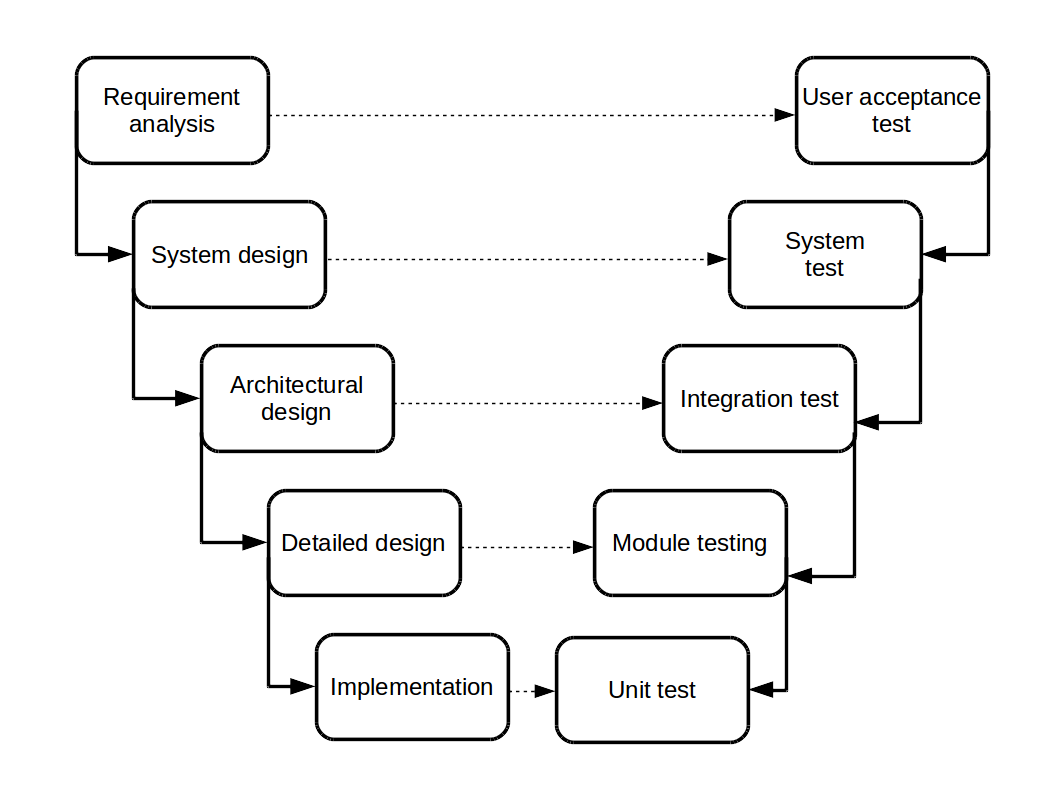
\includegraphics[width=1.0\textwidth]{figuras/vModel}
\caption{\label{fig:vModel}The V-model}
\end{figure}

The V-model shown in Figure \ref{fig:vModel} associates each level of testing to a different phase in the development process. This model is typically viewed as an extension of the waterfall methodology, but it does not imply the waterfall approach, since the synthesis and analysis activities can be applied to any development process \cite{Ammann:08}. 

\begin{itemize}

\item Requirement analysis phase: Customer's needs are registered. \textbf{User acceptance tests (UAT)} are constructed to check whether the delivered system meets the customer's requirements.

\item System design phase: Technical team analyses the captured requirements, studies the possible implementations and documents a technical specification. \textbf{System tests} are designed at this stage assuming that each component works accordingly and checks for the system to work as a whole.

\item Architectural design phase: Specify interface relationships, dependencies, structure and behaviour of subsystems. \textbf{Integration tests} are developed, with the assumption that each module works correctly, in order to verify all interfaces and communication among subsystems.

\item Detailed design phase: A low-level design is done to divide the system in smaller pieces, each of them with the corresponding behaviour specified so that the programmer can code. \textbf{Module testing} is designed to check each module individually.

\item Implementation phase: Code is actually produced. \textbf{Unit tests} are designed to test if every smallest unit of code, such as a method, can work correctly when isolated.
 
\end{itemize}

\subsection{Functional and Structural tests}

Testing techniques can be divided into functional and structural categories.

\subsubsection{Functional technique (black box)}
\label{funcTests}

The software behaviour described in the specification is considered to create the test cases. It is necessary to study the behaviour, develop the corresponding test cases, submit the system to the test cases and analyse the results observed comparing them to what was expected according to the description in the specification\cite{introSoftTest}:

	\begin{itemize}
	\item \textbf{Equivalence classes partitioning}
	
	Input data are partitioned into valid and invalid classes according to the conditions specified. The test cases are created based on each class by selecting an element in each class as a representative of the whole class. Using this criterion, the test cases can be executed systematically according to the requirements.

	\item \textbf{Analysis of the boundary value}
	
	Similar to the previous criterion, but the selection of the representative is done based on the classes' boundary. For that reason, the conditions associated with the limit values are exercised more strictly.

	\end{itemize}

Since many specifications are written in a descriptive fashion, the test cases developed using the functional technique can be very informal and not rigorous enough, which makes it difficult to automate their execution and human intervention becomes necessary. However, this technique only requires that requirements, input and corresponding output are identified. Thus, it can be applied during several testing phases, such as integration and system testing.

\subsubsection{Structural technique (white box)}
\label{strucTest}

The structure of the code implementation is considered to create the test cases in this category. In this technique, the program is represented by an oriented flow control graph, in which each node corresponds to a block of code (a statement in the code for instance) and each edge corresponds to a transition between blocks. The criteria related to this technique are concerned with the coverage of the program graph, such as \cite{Ammann:08}:

	\begin{itemize}
	\item \textbf{Node coverage}

	Every reachable node in the graph must be exercised by the test set. Node coverage is implemented by many testing tools, most often in the form of statement coverage
	
	\item \textbf{Edge coverage}

	Every edge in the graph must be tested in the test set.
	\item \textbf{Complete path coverage}

	All paths in the graph must be tested by the test set. This criterion is infeasible if there are cycles in the graph due to the infinity number of paths.

	\item \textbf{Prime path coverage}

	A path is a prime path if it is a simple path and it does not appear as a proper sub-path of any other simple path. In this criterion, all prime paths should be tested.

	\item \textbf{Specified Path Coverage}

	A specific set $S$ of paths is given and the test set must exercise all paths in $S$. This situation might occur if the use case scenarios provided by the customer are converted to paths in the graph and the team wishes to test them. 
	\end{itemize}

Tests obtained via the structural technique contribute specially to code maintenance and increase the reliability of the implementation. But, they do not represent a way to validate the system against the customer's requirements, since the specified requirements are not considered in their design.

%\subsection{Formal methods and tests}
